\exercisesheader{}

% 37

\eoce{\qt{Underage drinking, Part II\label{underage_drinking_normal_approx}} \videohref{ahss_eoce_sol-underage_drinking_normal_approx}\ \ 
We learned in Exercise~\ref{underage_drinking_intro}
that about 70\% of 18-20 year olds consumed alcoholic
beverages in any given year. We now consider a random 
sample of fifty 18-20 year olds.
\begin{parts}
\item How many people would you expect to have consumed alcoholic beverages? 
And with what standard deviation?
\item Would you be surprised if there were 45 or more people who have 
consumed alcoholic beverages?
\item What is the probability that 45 or more people in this sample have 
consumed alcoholic beverages? How does this probability relate to your answer 
to part (b)?
\end{parts}
}{}

% 38

\eoce{\qt{Chickenpox, Part II\label{chicken_pox_normal_approx}} We learned in 
Exercise~\ref{chicken_pox_intro} that about 90\% of American adults had 
chickenpox before adulthood. We now consider a random sample of 120 American 
adults.
\begin{parts}
\item How many people in this sample would you expect to have had chickenpox 
in their childhood? And with what standard deviation?
\item Would you be surprised if there were 105 people who have had chickenpox 
in their childhood?
\item What is the probability that 105 or fewer people in this sample have 
had chickenpox in their childhood? How does this probability relate to your 
answer to part (b)?
\end{parts}
}{}

% 39

\eoce{\qt{Game of dreidel\label{dreidel}} A dreidel is a four-sided spinning top 
with the Hebrew letters \textit{nun}, \textit{gimel}, \textit{hei}, and 
\textit{shin}, one on each side. Each side is equally likely to come up in a 
single spin of the dreidel. Suppose you spin a dreidel three times. Calculate 
the probability of getting

\noindent\begin{minipage}[c]{0.38\textwidth}
\begin{parts}
\item at least one \textit{nun}? 
\item exactly 2 \textit{nun}s? 
\item exactly 1 \textit{hei}? 
\item at most 2 \textit{gimel}s? \vspace{3mm}
\end{parts}
\end{minipage}%
\begin{minipage}[c]{0.32\textwidth}
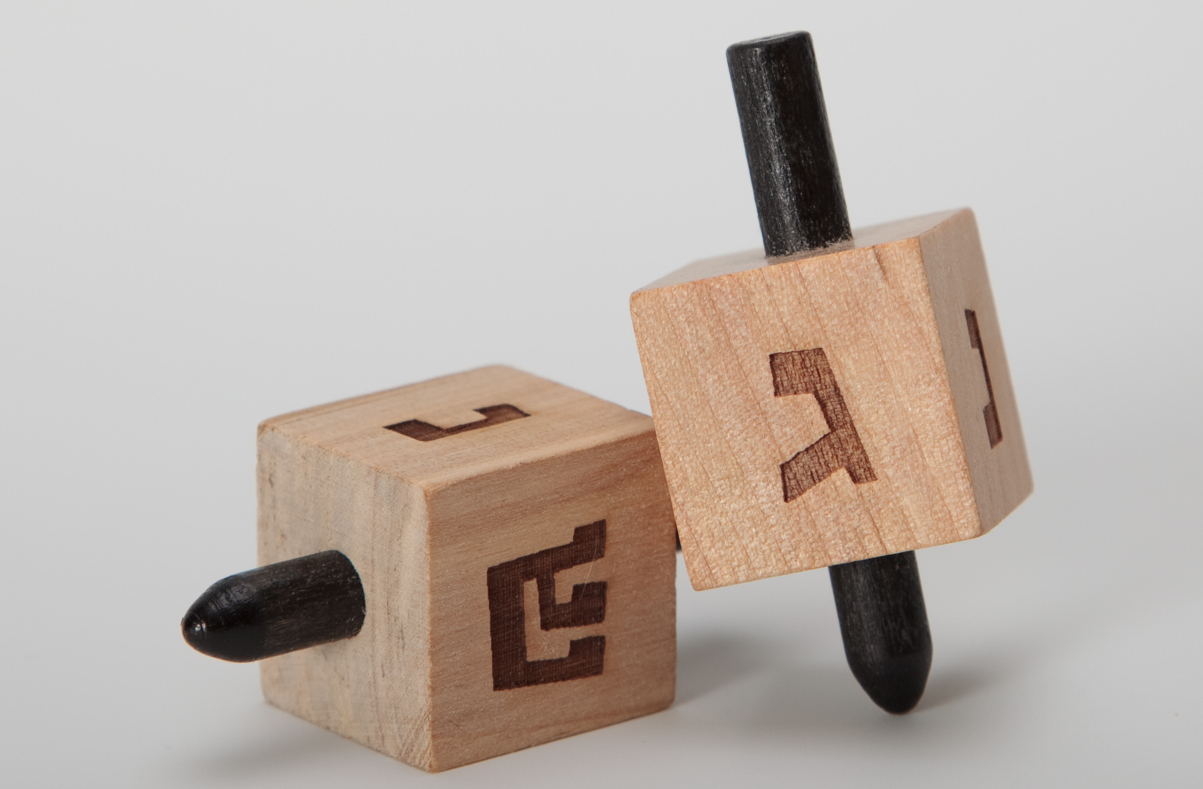
\includegraphics[width=0.9\textwidth]{ch_distributions/figures/eoce/dreidel/dreidel.jpg}
\end{minipage}%
\begin{minipage}[c]{0.28\textwidth}%
{\footnotesize Photo by Staccabees, cropped \\
  (\oiRedirect{textbook-flickr_staccabees_dreidels}{http://flic.kr/p/7gLZTf}) \\
  \oiRedirect{textbook-CC_BY_2}{CC~BY~2.0~license}} \\
\end{minipage}
}{}



% 40

\eoce{\qt{Sickle cell anemia\label{sickle_cell_anemia}} Sickle cell anemia is a 
genetic blood disorder where red blood cells lose their flexibility and 
assume an abnormal, rigid, ``sickle" shape, which results in a risk of 
various complications. If both parents are carriers of the disease, then a 
child has a 25\% chance of having the disease, 50\% chance of being a 
carrier, and 25\% chance of neither having the disease nor being a carrier. 
If two parents who are carriers of the disease have 3 children, what is the 
probability that 
\begin{parts}
\item two will have the disease?
\item none will have the disease?
\item at least one will neither have the disease nor be a carrier?
\item the first child with the disease will the be $3^{rd}$ child?
\end{parts}
}{}
